\chapter{Solid Mechanics
Model\index{SolidMechanicsModel}\label{sect:smm}}

The solid mechanics model is a specific implementation of the
\code{Model} interface dedicated to handle the equations of motion or
equations of equilibrium. The model is created for a given mesh.  It
will create its own \code{FEM} object to compute the interpolation,
gradient, integration and assembly operations.  A
\code{SolidMechanicsModel} object can simply be created like this:
\begin{cpp} SolidMechanicsModel model(mesh, spatial_dimension);
\end{cpp} where \code{mesh} is the mesh for which the equations are to
be solved, and \code{spatial\_dimension} is the dimensionality of the
problem.  If the \code{spatial\_dimension} is omitted, the problem is
assumed to have the same dimensionality as the one specified by the
mesh.

This model contains at least the the following six \code{Arrays}:
\begin{description}
\item[boundary] contains a boolean value for each degree of freedom
specifying whether that degree is blocked or not. A Dirichlet boundary
condition can be prescribed by setting the \textbf{boundary} value of
a degree of freedom to \code{true}.  A Neumann boundary condition can
be applied by setting the \textbf{boundary} value of a degree of
freedom to \code{false}.  The \textbf{displacement}, \textbf{velocity}
and \textbf{acceleration} are computed for all degrees of freedom for
which the \textbf{boundary} value is set to \code{false}. For the
remaining degrees of freedom, the imposed values (zero by default
after initialization) are kept.
\item[displacement] contains the displacements of all degrees of
freedom. It can be either a computed displacement for free degrees of
freedom or an imposed displacement in case of blocked ones ($\vec{u}$
in the following).
\item[velocity] contains the velocities of all degrees of freedom.  As
\textbf{displacement}, it contains computed or imposed velocities
depending on the nature of the degrees of freedom ($\vec{\dot{u}}$ in
the following).
\item[acceleration] contains the accelerations of all degrees of
freedom. As \textbf{displacement}, it contains computed or imposed
accelerations depending on the nature of the degrees of freedom
($\vec{\ddot{u}}$ in the following).
\item[force] contains the external forces applied on the nodes
($\vec{f_{\st{ext}}}$ in the following).
\item[residual] contains the difference between external and internal
forces. On blocked degrees of freedom, \textbf{residual} contains the
support reactions.  ($\vec{r}$ in the following).  It should be
mentioned that at equilibrium \textbf{residual} should be zero on free
degrees of freedom.
\end{description}

Some examples to help to understand how to use this model will be
presented in the next sections.

\section{Model setup}

\subsection{Setting initial
conditions \label{sect:smm:initial_condition}}

For a unique solution of the equations of motion initial displacements
and velocities at time $t=0$ at all degrees of freedom must be
specified:

\begin{eqnarray} \vec{u(t=0)} = \vec{u}_{0}\\ \vec{\dot u(t=0)} =
\vec{v}_{0}~.
\end{eqnarray} The solid mechanics model can be initialized as
follows:
\begin{cpp} model.initFull("material.dat")
\end{cpp} This function initializes the internal arrays and sets them
to zero. Initial displacements and velocities that are not equal to
zero can be prescribed by running a loop over the total number of
nodes. Here, the initial displacement and in x-direction and the
initial velocity in y-direction at all nodes is set to $0.1$ and $1$
respectively.
\begin{cpp} Array<Real> & disp = model.getDisplacement(); Array<Real>
& velo = model.getVelocity(); for (UInt i = 0; i < nb_nodes; ++i) {
disp(i, 0) = 0.1; velo(i, 1) = 1.; }
\end{cpp}

\subsection{Setting boundary conditions\label{sect:smm:boundary}} This
section explains how to impose Dirichlet or Neumann boundary
conditions. A Dirichlet boundary condition specifies the values that
the displacement needs to take for every point $x$ at the boundary
($\Gamma_u$) of the problem domain (Fig.~\ref{fig:smm:boundaries}):
\begin{equation} \vec{u} = \vec{\bar u} \quad \forall \vec{x}\in
\Gamma_{u}
\end{equation} A Neumann boundary condition specifies the values that
the gradient of the solution needs to take at the boundary
($\Gamma_t$) of the problem domain (Fig.~\ref{fig:smm:boundaries}):
\begin{equation} \vec{t} = \mat{\sigma} \vec{n} = \vec{\bar t} \quad
\forall \vec{x}\in \Gamma_{t}
\end{equation}
\begin{figure}[!htb] \centering
  \includegraphics[scale=0.6]{figures/boundary}
  \caption{Problem boundary in two
dimensions.\label{fig:smm:boundaries}}
\end{figure}

Different ways of imposing these boundary conditions exist. A basic
way is to loop over nodes or elements at the boundary and apply local
values. A more advanced method consists of using the notion of the
boundary of the mesh. In the following both ways are presented.

Starting with the basic approach, as mentioned the Dirichlet boundary
conditions can be applied by looping on the nodes and assigning the
required values. Figure~\ref{fig:smm:dirichlet_bc} shows a beam with a
fixed support on the left side. On the right end of the beam a load is
applied. At the fixed support, the displacement has a given value. For
this example, the displacement in both the x- and y-direction is set
to zero. Implementing this displacement boundary condition is similar
to the implementation of initial displacement conditions described
above. However, in order to impose a displacement boundary condition
for all time steps, the corresponding nodes need to be marked as
boundary nodes as shown in the following code:

 \begin{cpp} Array<bool> & boun = model.getBoundary();

  const Array<Real> & pos = mesh.getNodes();

  UInt nb_nodes = mesh.getNbNodes(); Real epsilon =
Math::getTolerance(); /* this tolerance is by default equal to the
machine precision but can be changed by using
%\code{Math::setTolerance(value)}% */

  for (UInt i = 0; i < nb_nodes; ++i) { if(std::abs(pos(i, 0)) <
epsilon) { boun(i, 0) = true; //block displacement in x-direction
boun(i, 1) = true; //block displacement in y-direction

      disp(i, 0) = 0.; //fixed displacement in x-direction disp(i, 1)
= 0.; //fixed displacement in y-direction } }
\end{cpp}
\begin{figure}[!htb] \centering
  \includegraphics[scale=0.4]{figures/dirichlet}
  \caption{Beam with fixed support.\label{fig:smm:dirichlet_bc}}
\end{figure}

For the more advanced approach, one needs the notion of a boundary in
the mesh. Therefore, the boundary should be created before boundary
condition functors can be applied. Generally the boundary can be
specified from the mesh file or the geometry.  For the first case, the
function \code{createBoundariesFromMeshDate} is called.  This function
can read any types of mesh data which are provided in the mesh
file. If the mesh file is created with Gmsh, the function takes one
input strings which is either \code{tag\_0, tag\_1} or
\code{physical\_names}. The first two tags are assigned by Gmsh to
each element which shows the physical group that they belong to. In
Gmsh, it is also possible to consider strings for different groups of
elements. These elements can be separated by giving a string
\code{physical\_names} to the function
\code{createBoundariesFromMeshData}.  Boundary conditions can also be
created from the geometry by calling
\code{createBoundariesFromGeometry}. This function gathers all the
elements on the boundary of the geometry.

To apply the required boundary conditions, the function \code{applyBC}
from the \code{SolidMechanicsModel} needs to be called. This function
gets a Dirichlet or Neumann functor and a string which specifies the
desired boundary on which the boundary conditions is to be
applied. The functors specify the type of conditions to apply. Three
build-in functors for Dirichlet exist: \code{FlagOnly, FixedValue,}
and \code{IncrementValue}. The functor \code{FlagOnly} is used if a
point is fixed in a given direction. Therefore, the input parameter to
this functor is only the fixed direction. The \code{FixedValue}
functor is used when a displacement value is applied in a fixed
direction. The \code{IncrementValue} applies an increment to the
displacement in a given direction. The following code shows the
utilization of three functors for the top, bottom and side surface of
the mesh which were already defined in the Gmsh file:

\begin{cpp}

 Boundary & boundary = mesh.getBoundary();
boundary.createBoundariesFromMeshData("physical_names");

  model.applyBC(BC::Dirichlet::FixedValue(13.0, BC::_y), "Top");

  model.applyBC(BC::Dirichlet::FlagOnly(BC::_x), "Bottom");

  model.applyBC(BC::Dirichlet::IncrementValue(13.0, BC::_x), "Side");

\end{cpp}

To apply a Neumann boundary condition, the applied traction or stress
should be specified before. In case of specifying the traction on the
surface, the functor \code{FromTraction} of Neumann boundary
conditions is called. Otherwise, the functor \code{FromStress} should
be called which gets the stress tensor as an input parameter.

\begin{cpp}

Array<Real> surface_traction(3); surface_traction(0)=0.0;
surface_traction(1)=0.0; surface_traction(2)=-1.0;

Array<Real> surface_stress(3, 3, 0.0); surface_stress(0,0)=0.0;
surface_stress(1,1)=0.0; surface_stress(2,2)=-1.0;

 model.applyBC(BC::Neumann::FromTraction(surface_traction), "Bottom");

 model.applyBC(BC::Neumann::FromStress(surface_stress), "Top");

\end{cpp}

If the boundary conditions needs to be removed in the simulation, a
functor is called from the Neumann boundary condition to free those
boundary conditions from the desired boundary.

\begin{cpp}

model.applyBC(BC::Neumann::FreeBoundary(), "Side");

\end{cpp}


User specified functors can also be implemented.  A full example for
setting both initial and boundary conditions can be found in
\shellcode{\examplesdir/boundary\_conditions.cc}.  The problem from
that example is shown in Fig.~\ref{fig:smm:bc_and_ic}. It consists of
a plate that is fixed with movable supports on the left and bottom
side. On the right side, a traction which increases linearly with the
number of time steps, is applied. The initial displacement and
velocity in x-direction at all free nodes is zero and two
respectively.
\begin{figure}[!htb] \centering
  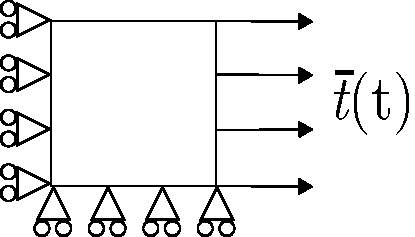
\includegraphics[scale=0.8]{figures/bc_and_ic_example}
  \caption{Plate on movable supports.\label{fig:smm:bc_and_ic}}
\end{figure}

\subsection{Material selector\label{sect:smm:materialselector}}

If the user wants to assign different materials to the different finite elements of the choice in Akantu, a material selector has to be used. There are four different material selectors defined in Akantu.

\begin{enumerate}
\item \code{MaterialSelector}: This material selector assigns a material to a specific element using an index value. If an index is not specified, it is using 0, hence the first material as default.
\item \code{DefaultMaterialSelector}: This selector assigns materials based on the values in the \code{element\_index\_by\_material} array.
\item \code{MeshDataMaterialSelector}: This material selector class uses mesh data information to assing different materials. With the proper tag name and index, different materials can be assigned as demonstrated in the example below.
\item \code{DefaultMaterialCohesiveSelector}: This is the default material selector for the cohesive elements and it inherits its properties from \code{DefaultMaterialSelector}. The material ID of the first cohesive element is extracted and assigned to all cohesive elements.
\end{enumerate}

Apart from the material selectors that are default in Akantu, users can always develop their own classes in the main code to tackle with various multi-material assignment situations.

For example, an application of \code{MeshDataMaterialSelector} will look like this:

\begin{cpp}
MeshDataMaterialSelector<UInt> * mat_selector;
mat_selector = new MeshDataMaterialSelector<UInt>("tag_1", model, 1);
model.setMaterialSelector(*mat_selector);
\end{cpp}

where \code{tag\_1} of the mesh file is used as the classifier index and the elements that have index value equal to one will be assigned to the first material in the material file.

\section{Static analysis\label{sect:smm:static}}

The \code{SolidMechanicsModel} class can handle different analysis
methods, the first one being presented is the static case.  In this
case, the equation to solve is,
\begin{equation}\label{eqn:smm:static} \mat{K} \vec{u} =
\vec{f_{\st{ext}}}~,
\end{equation} where $\mat{K}$ is the global stiffness matrix,
$\vec{u}$ the displacement vector and $\vec{f_{\st{ext}}}$ the
external forces vector applied to the system.


To solve such a problem the static solver of the
\code{SolidMechanicsModel}\index{SolidMechanicsModel} object is used.
First a model has to be created and initialized.  To create the model,
a mesh that can be read from a file is needed, as explained in section
\ref{sect:common:mesh}.  Once an instance of a
\code{SolidMechanicsModel} is obtained, the easiest way to initialize
it is to use the \code{initFull}\index{SolidMechanicsModel!initFull}
function by giving the \code{SolidMechanicsModelOptions}. These
options allow to decide which type of analysis should be used and if
the materials should be initialized or not.
\begin{cpp} SolidMechanicsModel model(mesh);
model.initFull(SolidMechanicsModelOptions(_static));
\end{cpp} Here the static analysis is chosen by passing the function
argument (\_static). By default the boolean for no initialization of
the materials is set to false, so that they are initialized during the
\code{initFull}. By calling \code{initFull} also all the needed
vectors are initialized to zero.  Once the model is created and
initialized the boundary conditions can be set as explained in section
\ref{sect:smm:boundary}.  Boundary conditions will prescribe the
external forces for the free degrees of freedom $\vec{f_{\st{ext}}}$
and displacements for the others.  At this point of the analysis the
function \code{solveStep}\index{SolidMechanicsModel!solveStep} can be
called:
\begin{cpp} model.solveStep<_scm_newton_raphson_tangent_modified,
_scc_residual>(1e-4, 1);
\end{cpp} This function is templated by the solving method and the
convergence criterion and takes two arguments, the tolerance and the
maximum number of iterations, which are $1e-4$ and $1$ for this
example. The modified Newton-Raphson method is chosen to solve the
system. In this method the equilibrium equation (\ref{eqn:smm:static})
is modified in order to apply a Newton-Raphson convergence algorithm:

\begin{align}\label{eqn:smm:static-newton-raphson} \mat{K}^{i+1}
\delta\vec{u}^{i+1} &= \vec{r} \\ &= \vec{f_{\st{ext}}} -
\vec{f_{\st{int}}}\\ &= \vec{f_{\st{ext}}} - \mat{K}^{i} \vec{u}^{i}\\
\vec{u}^{i+1} &= \vec{u}^{i} + \delta\vec{u}^{i+1}~,\nonumber
\end{align}
where $\delta\vec{ u}$ is the increment of displacement to be added
from one iteration to the other, and $i$ is the number of the
Newton-Raphson iteration.  By invoking the \code{solveStep} function
in the first step the global stiffness matrix $\mat{K}$ from equation
(\ref{eqn:smm:static}) is automatically assembled. A Newton-Raphson
iteration is subsequently started, $\mat{K}$ is updated according to
the displacement computed at the previous iteration and one loops
until the forces are balanced (\_scc\_residual), \ie $\vec{r} = 0$.
One can also iterate until the increment of displacement is zero
(\_scc\_increment) which also means that the equilibrium is found.
For an elastic problem the solution is directly found at the first
iteration and therefore the maximum number of iterations can be set to
one. But for a non-elastic case, one needs to iterate as long as the
norm of the residual is not zero and therefore the maximum number of
iterations has to be higher, \textit{e.g.} $100$:
\begin{cpp} model.solveStep<_scm_newton_raphson_tangent_modified,
_scc_residual>(1e-4, 100);
\end{cpp} At the end of the analysis the final solution is stored in
the \textbf{displacement} vector.  A full example of how to solve a
static problem is presented in the code
\code{\examplesdir/static/static.cc}.  This example is composed of a
2D plate of steel, blocked with rollers on the left and bottom sides
as shown in Figure \ref{fig:smm:static}.  The nodes from the right
side of the sample are displaced by $0.01\%$ of the length of the
plate.

\begin{figure}[!htb] \centering
  \includegraphics{figures/static}
  \caption{Numerical setup\label{fig:smm:static}}
\end{figure}

The results of this analysis is depicted in Figure
\ref{fig:smm:implicit:static_solution}.

\begin{figure}[!htb] \centering
  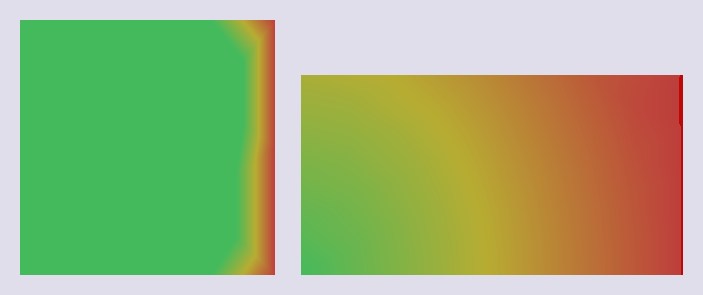
\includegraphics[width=.6\linewidth]{figures/static_analysis}
  \caption{Solution of the static analysis. Left: the initial
condition, right: the solution (deformation magnified 50 times)}
  \label{fig:smm:implicit:static_solution}
\end{figure}

\section{Dynamic methods} \label{sect:smm:Dynamic_methods}

Different ways to solve the equations of motion are implemented in the
solid mechanics model.  The complete equations that should be solved
are:
\begin{equation}\label{eqn:equation-motion} \mat{M}\vec{\ddot{u}} +
\mat{C}\vec{\dot{u}} + \mat{K}\vec{u} = \vec{f_{\st{ext}}} -
\vec{f_{\st{int}}} = \vec{r}~,
\end{equation} where $\mat{M}$, $\mat{C}$ and $\mat{K}$ are the mass,
damping and stiffness matrices, respectively.

In the previous section, it has already been discussed how to solve
this equation in the static case where $\vec{\ddot{u}} = \vec{\dot{u}}
= 0$.  Here the method to solve this equation in the general case will
be presented.  For this purpose, a time discretization should be
added.  The most common discretization method in solid mechanics is
the Newmark-$\beta$ method, which is therefore also the default in
\akantu.

For the Newmark-$\beta$ method, equation (\ref{eqn:equation-motion})
becomes a system of three equations (see \cite{curnier92a}
\cite{hughes-83a} for more detail):
\begin{align} \mat{M} \vec{\ddot{u}}_{n+1} + \mat{C}
\vec{\dot{u}}_{n+1} + \mat{K} \vec{u}_{n+1} &=
\vec{r}_{n+1} \label{eqn:equation-motion-discret} \\ \vec{u}_{n+1} &=
\vec{u}_{n} + \left(1 - \alpha\right) \Delta t \vec{\dot{u}}_{n} +
\alpha \Delta t \vec{\dot{u}}_{n+1} + \left(\frac{1}{2} -
\alpha\right) \Delta t^2
\vec{\ddot{u}}_{n} \label{eqn:finite-difference-1}\\
\vec{\dot{u}}_{n+1} &= \vec{\dot{u}}_{n} + \left(1 - \beta\right)
\Delta t \vec{\ddot{u}}_{n} + \beta \Delta t
\vec{\ddot{u}}_{n+1} \label{eqn:finite-difference-2}
\end{align}

In this new equations, $\vec{\ddot{u}}_{n}$, $\vec{\dot{u}}_{n}$ and
$\vec{u}_{n}$ are the approximations of $\vec{\ddot{u}(t_n)}$,
$\vec{\dot{u}(t_n)}$ and $\vec{u(t_n)}$.  Equation
(\ref{eqn:equation-motion-discret}) is the equation of motion in terms
of approximate solution and the equations
(\ref{eqn:finite-difference-1}) and (\ref{eqn:finite-difference-2})
are the finite difference formulas describing the evolution of the
approximate solutions.  The $\alpha$ and $\beta$ parameters determine
the stability and the accuracy of the algorithm. Classical values for
$\alpha$ and $\beta$ are usually $\beta = 1/2$ for no numerical
damping and $0 < \alpha < 1/2$.

\begin{center}
  \begin{tabular}{cll} \toprule $\alpha$ & Method ($\beta = 1/2$) &
Type\\ \midrule $0$ & central difference & explicit\\ $1/6$ &
Fox-Goodwin (royal road) &implicit\\ $1/3$ & Linear acceleration
&implicit\\ $1/2$ & Average acceleration (trapezoidal rule)&
implicit\\ \bottomrule
  \end{tabular}
\end{center}

To be able to solve this system of equations,
(\ref{eqn:equation-motion-discret})-(\ref{eqn:finite-difference-2})
should be split in a predictor-corrector system of equations.
Moreover, in the case of a non-linear equation as for the static case,
an iterative algorithm such as the Newton-Raphson method is applied.
According to these conditions, the system of equations can be written
as:


\noindent\textit{Predictor:}
\begin{align} \vec{u}_{n+1}^{0} &= \vec{u}_{n} + \Delta t
\vec{\dot{u}}_{n} + \frac{\Delta t^2}{2} \vec{\ddot{u}}_{n} \\
\vec{\dot{u}}_{n+1}^{0} &= \vec{\dot{u}}_{n} + \Delta t
\vec{\ddot{u}}_{n} \\ \vec{\ddot{u}}_{n+1}^{0} &= \vec{\ddot{u}}_{n}
\end{align}

\noindent\textit{Solve:}
\begin{align} \left(c \mat{M} + d \mat{C} + e \mat{K}_{n+1}^i\right)
\vec{w} = \vec{f_{\st{ext}}}_{n+1} - \vec{f_{\st{int}}}_{n+1}^i -
\mat{C} \vec{\dot{u}}_{n+1}^i - \mat{M} \vec{\ddot{u}}_{n+1}^i
\end{align}

\noindent\textit{Corrector:}
\begin{align} \vec{\ddot{u}}_{n+1}^{i+1} &= \vec{\ddot{u}}_{n+1}^{i} +
c \vec{w} \\ \vec{\dot{u}}_{n+1}^{i+1} &= \vec{\dot{u}}_{n+1}^{i} + d
\vec{w} \\ \vec{u}_{n+1}^{i+1} &= \vec{u}_{n+1}^{i} + e \vec{w}
\end{align}

where $i$ is the Newton-Raphson iteration counter and $c$, $d$ and $e$
are parameters depending on the method used to solve the equations

\begin{center}
  \begin{tabular}{lcccc} \toprule & $\vec{w}$ & $e$ & $d$ & $c$\\
\midrule in acceleration &$ \delta\vec{\ddot{u}}$ & $\alpha \beta
\Delta t^2$ &$\beta \Delta t$ &$1$\\ in velocity & $
\delta\vec{\dot{u}}$& $\frac{1}{\beta} \Delta t$ & $1$ & $\alpha
\Delta t$\\ in displacement &$\delta\vec{u}$ & $ 1$ &
$\frac{1}{\alpha} \Delta t$ & $\frac{1}{\alpha \beta} \Delta t^2$\\
\bottomrule
  \end{tabular}
\end{center}

\note{If you want to use the implicit solver \akantu should be
compiled at least with one sparse matrix solver such as
Mumps\cite{mumps}.}


\subsection{Implicit time integration} To solve a problem with an
implicit time integration scheme, first a \code{SolidMechanicsModel}
object should be created and initialized.  Then the initial and
boundary conditions have to be set.  Everything is similar to the
example in the static case (section \ref{sect:smm:static}), however,
in this case during the initialization of the model, the implicit
dynamic case should be selected.

\begin{cpp} SolidMechanicsModel model(mesh);
model.initFull(SolidMechanicsModelOptions(_implicit_dynamic)); /*
Boundary conditions see section %\ref{sect:smm:boundary}% */
\end{cpp} Since a dynamic simulation is conducted, a time step $\Delta
t$ has to be specified. In the case of implicit simulations, \akantu
implements a trapezoidal rule by default.  That is to say $\alpha =
1/2$ and $\beta = 1/2$ which is unconditionally stable. Therefore the
value of the time step can be chosen arbitrarily.
\index{SolidMechanicsModel!setTimeStep}
\begin{cpp} model.setTimeStep(time_step);
\end{cpp} Since the system has to be solved a for a given amount of
time steps the function \code{solveStep()}, which has already been
used in the static example \ref{sect:smm:static}, has to be called
inside a time loop:
\begin{cpp} /// time loop Real time = 0.; for (UInt s = 1; time <
max_time; ++s, time += time_step) {

    model.solveStep<_scm_newton_raphson_tangent_modified,
_scc_increment>(1e-12, 100); }
\end{cpp} An example of solid mechanics with a implicit time scheme is
presented in \shellcode{\examplesdir/implicit/implicit\_dynamic.cc}.
This example consists of a 3D beam of
$\unit{10}{\meter}\,\times\,\unit{1}{\meter}\,\times\,\unit{1}{\meter}$
blocked on one side and is on a roller on the other side.  A constant
force of \unit{5}{\kilo\newton} is applied in the middle of this beam.
Figure \ref{fig:smm:implicit:dynamic} presents the geometry of this
case. The material used is a linear fictitious elastic material with a
density of \unit{1000}{\kilogrampercubicmetre}, a Young's Modulus of
\unit{120}{\mega\pascal} and Poisson's ratio of $0.3$. These values
were chosen to simplify the analytical solution.

An approximation of the dynamic response of the middle point of the
beam is given by:
\begin{equation}\label{eqn:smm:implicit} u\left(\frac{L}{2}, t\right)
= \frac{1}{\pi^4} \left(1 - cos\left(\pi^2 t\right) +
\frac{1}{81}\left(1 - cos\left(3^2 \pi^2 t\right)\right) +
\frac{1}{625}\left(1 - cos\left(5^2 \pi^2 t\right)\right)\right)
\end{equation}

\begin{figure}[!htb] \centering
  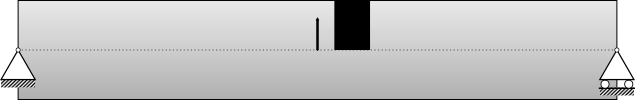
\includegraphics[scale=.6]{figures/implicit_dynamic}
  \caption{Numerical setup}
  \label{fig:smm:implicit:dynamic}
\end{figure}

Figure \ref{fig:smm:implicit:dynamic_solution} presents the deformed
beam at 3 different times of the simulation, time steps 0, 1000 and
2000.

\begin{figure}[!htb] \centering \setlength{\unitlength}{0.1\textwidth}
  \begin{tikzpicture} \node[above right] (img) at (0,0)
{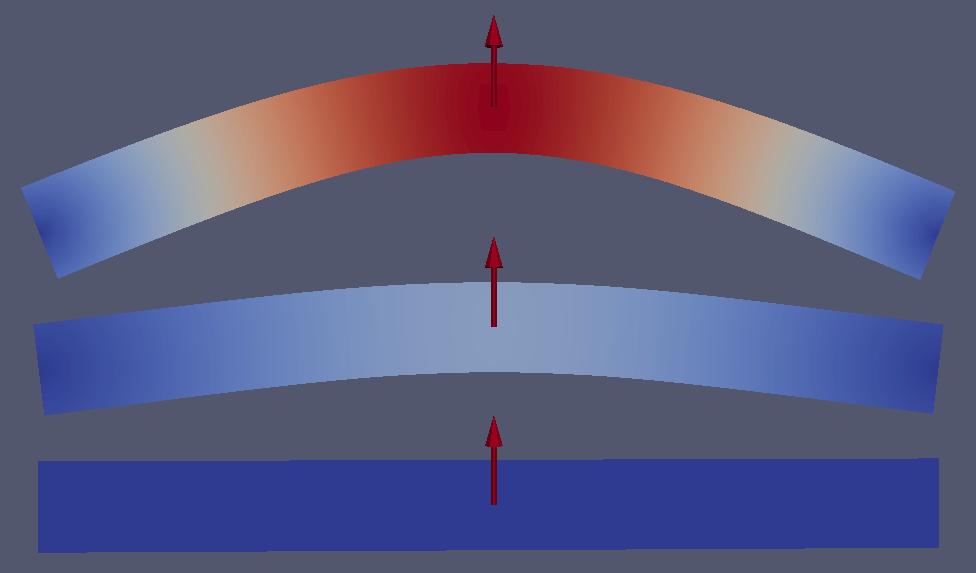
\includegraphics[width=.6\linewidth]{figures/dynamic_analysis}};
\node[left] at (0pt,20pt) {$0$}; \node[left] at (0pt,60pt) {$1000$};
\node[left] at (0pt,100pt) {$2000$};
  \end{tikzpicture}

  \caption{Deformed beam at 3 different time (displacement are
magnified by a factor 10).}
  \label{fig:smm:implicit:dynamic_solution}
\end{figure}

\subsection{Explicit dynamic}

The explicit dynamic time integration scheme is based on the
Newmark-$\beta$ scheme with $\alpha=0$ (see equations
\ref{eqn:equation-motion-discret}-\ref{eqn:finite-difference-2}).  In
\akantu, $\beta$ is defined as $\beta=1/2$, see section
\ref{sect:smm:Dynamic_methods}.

The initialization of the simulation is similar to the static and
implicit dynamic version.  The model is created from the
\code{SolidMechanicsModel} class.  In the initialization, the use of
the explicit scheme should be defined with the
\code{\_explicit\_dynamic} keyword.

\begin{cpp} SolidMechanicsModel model(mesh);
model.initFull(SolidMechanicsModelOptions(_explicit_lumped_mass));
\end{cpp} \index{SolidMechanicsModel!initFull}

\note{Writing \code{model.initFull(SolidMechanicsModelOptions());} is
equivalent to use the \code{\_explicit\_lumped\_mass} keyword, as this
is the default case.}

The implemented explicit time integration scheme in \akantu uses a
lumped mass matrix $\mat{M}$ (reducing the computational cost). This
matrix is assembled by distributing the mass of each element onto its
nodes. The resulting $\mat{M}$ is therefore a diagonal matrix stored
in the \textbf{mass} vector of the model.


\begin{cpp} model.assembleMassLumped();
\end{cpp} \index{SolidMechanicsModel!assembleMassLumped}

The explicit integration scheme is conditionally stable. The time step
has to be smaller than the stable time step which is obtained in
\akantu as follows:

\begin{cpp} time_step = model.getStableTimeStep();
\end{cpp} \index{SolidMechanicsModel!StableTimeStep}

The stable time step is defined as:
\begin{equation}\label{eqn:smm:explicit:stabletime} \Delta
t_{\st{crit}} = \Delta x \sqrt{\frac{\rho}{2 \mu + \lambda}}
\end{equation} where $\Delta x$ is a characteristic length (\eg the
inradius in the case of linear triangle element), $\mu$ and $\lambda$
are the first and second Lame's coefficients and $\rho$ is the
density.  The stable time step corresponds to the time the fastest
wave (the compressive wave) needs to travel the characteristic length
of the mesh.  However, note that if the time step of the computation
is equal to the stable time step, the simulation remains
unstable. Therefore, it is necessary to impose a time step that is
smaller than the stable time step, for instance, by multiplying the
stable time step by a safety factor smaller than one.

\begin{cpp} const Real safety_time_factor = 0.1; Real
applied_time_step = time_step * safety_time_factor;
model.setTimeStep(applied_time_step);
\end{cpp} \index{SolidMechanicsModel!setTimeStep}

The initial displacement and velocity fields are, by default, equal to
zero if not given specifically by the user (see
\ref{sect:smm:initial_condition}).

Like in implicit dynamics a time loop is used in which the
displacement, velocity and acceleration fields are updated at each
time step. The values of these fields are obtained from the
Newmark$-\beta$ equations with $\beta=1/2$ and $\alpha=0$. In akantu
these computations at each time step are invoked by calling the
function \code{solveStep}:
\begin{cpp} for (UInt s = 1; (s-1)*applied_time_step < total_time;
++s) { model.solveStep(); }
\end{cpp} \index{SolidMechanicsModel!solveStep} The function
\code{solveStep} wraps the four following functions:
\begin{itemize}
\item \code{model.explicitPred()} allows to compute the displacement
field at $t+1$ and a part of the velocity field at $t+1$, denoted by
$\vec{\dot{u}_{n+1/2}}$, which will be used later in the
\code{model.explicitCorr()}. The solved equations are:

  \begin{align} \vec{u}_{n+1} &= \vec{u}_{n} + \Delta t
\vec{\dot{u}}_{n} + \frac{\Delta t^2}{2} \vec{\ddot{u}}_{n}\\
\vec{\dot{u}_{n+1/2}} &= \vec{\dot{u}}_{n} + \Delta t
\vec{\ddot{u}}_{n}
    \label{eqn:smm:explicit:onehalfvelocity}
  \end{align}

\item \code{model.updateResidual()} and
\code{model.updateAcceleration()} allow to solve the equation which
gives the acceleration increment $\delta \vec{\ddot{u}}$:

  \begin{equation} \left(\mat{M} + \frac{1}{2} \Delta t \mat{C}\right)
\delta \vec{\ddot{u}} = \vec{f_{\st{ext}}} - \vec{f}_{\st{int}n+1} -
\mat{C} \vec{\dot{u}}_{n} - \mat{M} \vec{\ddot{u}}_{n}
  \end{equation}

  \note{The internal force $\vec{f}_{\st{int}n+1}$ is computed from
the displacement $\vec{u}_{n+1}$ based on the constitutive law.}

\item \code{model.explicitCorr()} computes the velocity and
acceleration fields at $t+1$:

  \begin{align} \vec{\dot{u}}_{n+1} &= \vec{\dot{u}}_{n+1/2} +
\frac{\Delta t}{2} \delta \vec{\ddot{u}} \\ \vec{\ddot{u}}_{n+1} &=
\vec{\ddot{u}}_{n} + \delta \vec{\ddot{u}}
  \end{align}
\end{itemize}

The use of the explicit time integration scheme is illustrated by an
example (see \code{\examplesdir/explicit/explicit\_dynamic.cc}).  This
example models the propagation of a wave in a steel beam. The beam is
blocked on one side and a displacement is applied on the other side,
as shown in figure \ref{fig:smm:explicit}.

\begin{figure}[!htb] \centering
  \includegraphics[scale=.6]{figures/explicit_dynamic}
  \caption{Numerical setup \label{fig:smm:explicit}}
\end{figure}

The length and height of the beam are \unit{10}{\metre} and
\unit{1}{\metre}, respectively.  The material is linear elastic,
homogeneous and isotropic (density:
\unit{7800}{\kilogrampercubicmetre}, Young's modulus:
\unit{210}{\giga\pascal} and Poisson's ratio: $0.3$).  The imposed
displacement is equal to $\Delta u = \unit{0.05}{\metre}$. The
potential, kinetic and total energies are computed.  The time factor
is equal to $0.1$.  The total simulated time is \unit{0.01}{\second}.

\section{Constitutive laws \label{sect:smm:CL}}\index{Material} In
order to compute an element's response to deformation, one needs to
use an appropriate constitutive relationship for every element in the
mesh. The constitutive law enables to compute the element's stresses
from the element's strains.

In the finite element discretization, the constitutive formulation is
applied to every quadrature point of each element. When the implicit
formulation used, the tangent matrix has to be computed. Every
constitutive law also provides the formulation required to compute the
tangent matrix.

The chosen materials for the virtual simulation have to be specified
in the mesh file or as an alternative they can be assigned using the
\code{element\_material} vector.  For every material assigned to the
problem one has to specify the material characteristics (constitutive
behavior and material properties) in a text file (\eg material.dat) as
follows:
\begin{cpp} material %\emph{constitutive\_law}% [ name = %\emph{XXX}%
rho = %\emph{XXX}% ...  ]
\end{cpp} \index{Constitutive\_laws} where \emph{constitutive\_law} is
the adopted constitutive law, followed by the material properties
listed one by line in the bracket (\eg \code{name} and density
\code{rho}). The file needs to be loaded in \akantu using the
\code{readMaterials} method
\begin{cpp} model.readMaterials("material.dat");
\end{cpp} or in alternative the \code{initFull} method.
\begin{cpp} model.initFull("material.dat");
\end{cpp} The following sections describe the constitutive models
implemented in \akantu.

\subsection{Elastic}\index{Material!Elastic} The elastic law is a
commonly used constitutive relationship that can be used for a wide
range of engineering materials (\eg metals, concrete, rock, wood,
glass, rubber, etc.) provided that the strains remain small (\ie small
deformation and stress lower than yield strength). The linear elastic
behavior is described by Hooke's law, which states that the stress is
linearly proportional to the applied strain (material behaves like an
ideal spring), as illustrated in Figure~\ref{fig:smm:cl:elastic}.
\begin{figure}[!htb]
  \begin{center}

    \subfloat[]{
      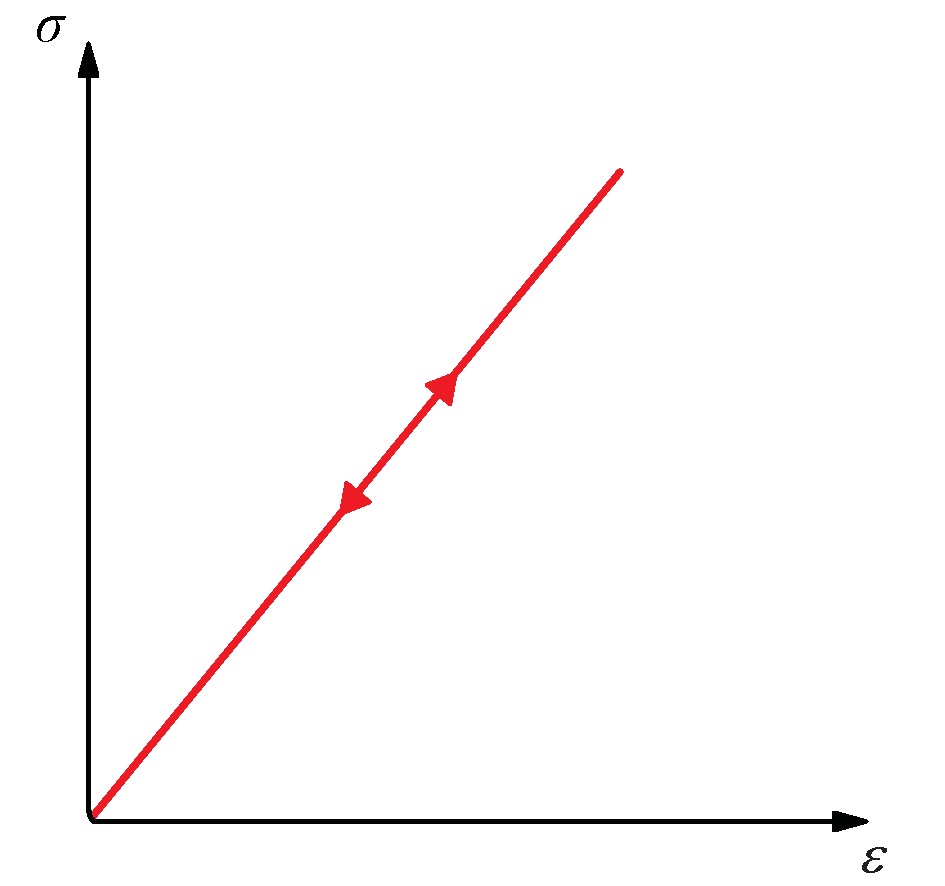
\includegraphics[width=0.4\textwidth,keepaspectratio=true]{figures/stress_strain_el.pdf}
      \label{fig:smm:cl:elastic:stress_strain} }
\hspace{0.05\textwidth} \subfloat[]{
\raisebox{0.125\textwidth}{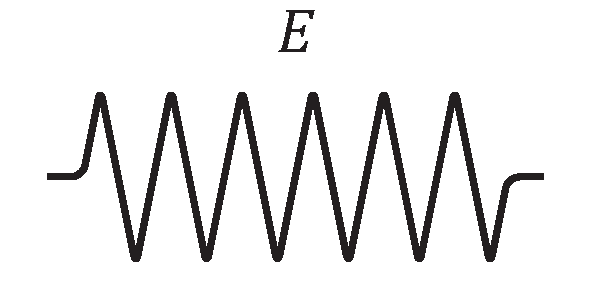
\includegraphics[width=0.25\textwidth,keepaspectratio=true]{figures/hooke_law.pdf}}
      \label{fig:smm:cl:elastic:hooke} }
    \caption{(a) Stress-strain curve for elastic material and (b)
schematic representation of Hooke's law, denoted as a spring.}
    \label{fig:smm:cl:elastic}
  \end{center}
\end{figure} The equation that relates the strains to the
displacements is: % First the strain is computed (at every gauss
point) from the displacements as follows:
\begin{equation}\label{eqn:smm:strain_inf} \mat{\epsilon} =
\frac{1}{2} \left[ \mat{F}-\mat{I}+(\mat{F}-\mat{I})^T \right]
\end{equation} where $\mat{\epsilon}$ represents the infinitesimal
strain tensor, $\mat{F} = \nabla_{\!\!\vec{X}}\vec{x}$ the deformation
gradient tensor and $\mat{I}$ the identity matrix. The constitutive
equation for isotropic homogeneous media can be expressed as:
\begin{equation}\label{eqn:smm:material:constitutive_elastic}
\mat{\sigma } =\lambda\mathrm{tr}(\mat{\epsilon})\mat{I}+2 \mu
\mat{\epsilon}
\end{equation} where $\mat{\sigma}$ is the Cauchy stress tensor
($\lambda$ and $\mu$ are the the first and second Lame's
coefficients). Besides the name and density, one has to specify the
following properties in the material file: \code{E} (Young's modulus),
\code{nu} (Poisson's ratio) and (for 2D) \code{Plane\_Stress} (if set
to zero or not specified plane strain conditions are assumed for a
plain analysis, otherwise plane stress conditions are applied).


\IfFileExists{manual-extra_materials.tex}{% \subsubsection{Caughey}
% ** Not in  release ** The model  is a particular case of  the Rayleigh damping
% model,   with    damping   being   proportional   only    to   the   stiffness
% matrix. Substitute with complete Rayleigh damping model for release?

\subsection{Neo-Hookean}\index{Material!Neohookean}

The hyperelastic Neo-Hookean constitutive law results from an
extension of the linear elastic relationship (Hooke's Law) for large
deformation. Thus, the model predicts nonlinear stress-strain behavior
for bodies undergoing large deformations.

\begin{figure}[!htb]
  \begin{center}
    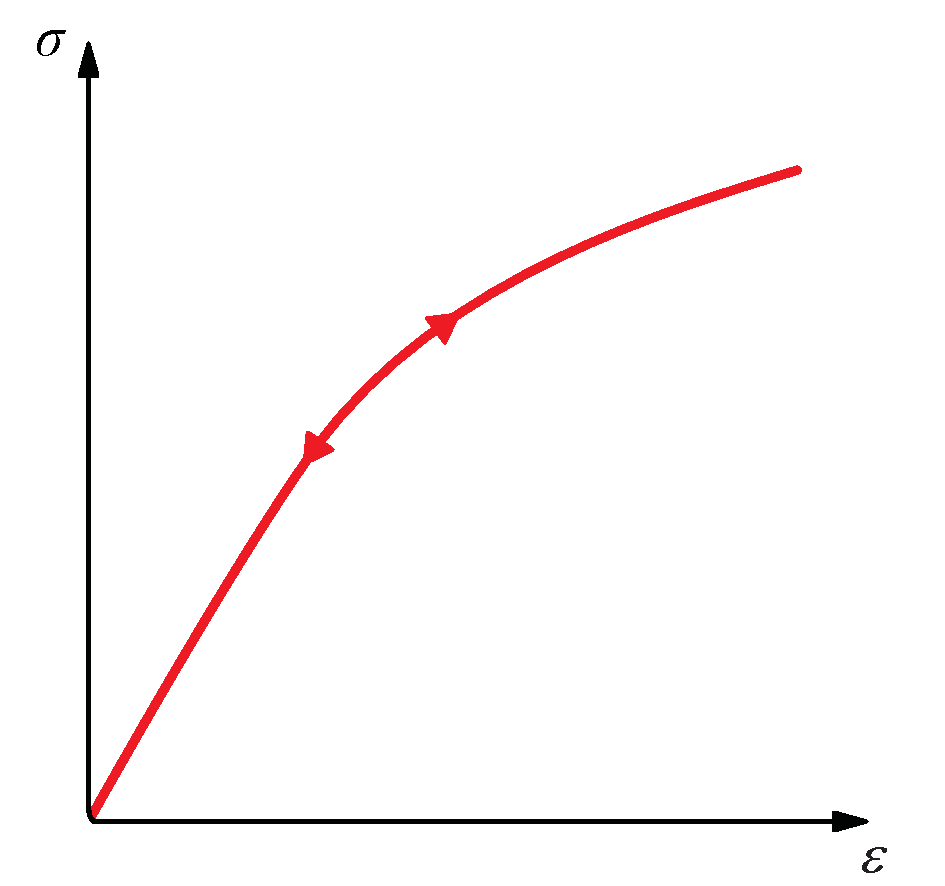
\includegraphics[width=0.4\textwidth,keepaspectratio=true]{figures/stress_strain_neo.pdf}
    \caption{Neo-hookean Stress-strain curve.}
    \label{fig:smm:cl:neo_hookean}
  \end{center}
\end{figure}

As illustrated in Figure~\ref{fig:smm:cl:neo_hookean}, the behavior is initially
linear and the mechanical behavior is very close to the corresponding linear
elastic material. This constitutive relationship, which accounts for compressibility,
 is a modified version of the one proposed by Ronald Rivlin \cite{Belytschko:2000}.

The strain energy stored in the material is given by:
\begin{equation}\label{eqn:smm:constitutive:neohookean_potential}
  \Psi(\mat{C}) = \frac{1}{2}\lambda_0\left(\ln J\right)^2-\mu_0\ln J+\frac{1}{2}
\mu_0\left(\text{trace}(\mat{C})-3\right)
\end{equation}
\noindent where $\lambda_0$ and $\mu_0$ are, respectively, Lamé's first parameter
and the shear modulus at the initial configuration. $J$ is the jacobian of the deformation
gradient ($\mat{F}=\nabla_{\!\!\vec{X}}\vec{x}$): $J=\text{det}(\mat{F})$. Finally $\mat{C}$ is the right Cauchy-Green
deformation tensor.

Since this kind of material is used for large deformation problems, a
finite deformation framework should be used. Therefore, the Cauchy
stress ($\mat{\sigma}$) should be computed through the second
Piola-Kirchhoff stress tensor $\mat{S}$:

\begin{equation}
  \mat{\sigma } = \frac{1}{J}\mat{F}\mat{S}\mat{F}^T
\end{equation}

Finally the second Piola-Kirchhoff stress tensor is given by:

\begin{equation}
  \mat{S}  = 2\frac{\partial\Psi}{\partial\mat{C}} = \lambda_0\ln J
\mat{C}^{-1}+\mu_0\left(\mat{I}-\mat{C}^{-1}\right)
\end{equation}

The parameters to indicate in the material file are the same
as those for the elastic case: \code{E} (Young's modulus), \code{nu} (Poisson's
ratio).

\subsection{Small-Deformation Plasticity}\index{Material!Small-deformation Plasticity}


The small-deformation plasticity is a simple plasticity material
formulation which accounts for the additive decomposition of strain
into elastic and plastic strain components. This formulation is
applicable to infinitesimal deformation where the additive
decomposition of the strain is a valid approximation. In this
formulation, plastic strain is a shearing process where hydrostatic
stress has no contribution to plasticity and consequently plasticity
does not lead to volume change. Figure ~\ref{fig:Lin-strain-hard}
shows the linear strain hardening elasto-plastic behavior according to
the additive decomposition of strain into the elastic and plastic
parts in infinitesimal deformation as


\begin{equation} \label{eqn:smm:constitutive:strain decomposition}
	\mat{\varepsilon} = \mat{\varepsilon}^e +\mat{\varepsilon}^p
\end{equation}  
\begin{equation} \label{eqn:smm:constitutive:Hooks law}
	{\mat{\sigma}} = 2G(\mat{\varepsilon}^e) + \lambda  trace(\mat{\varepsilon}^e)\mat{I}
\end{equation}

\noindent 
\begin{figure}[htp]
  \centering
   {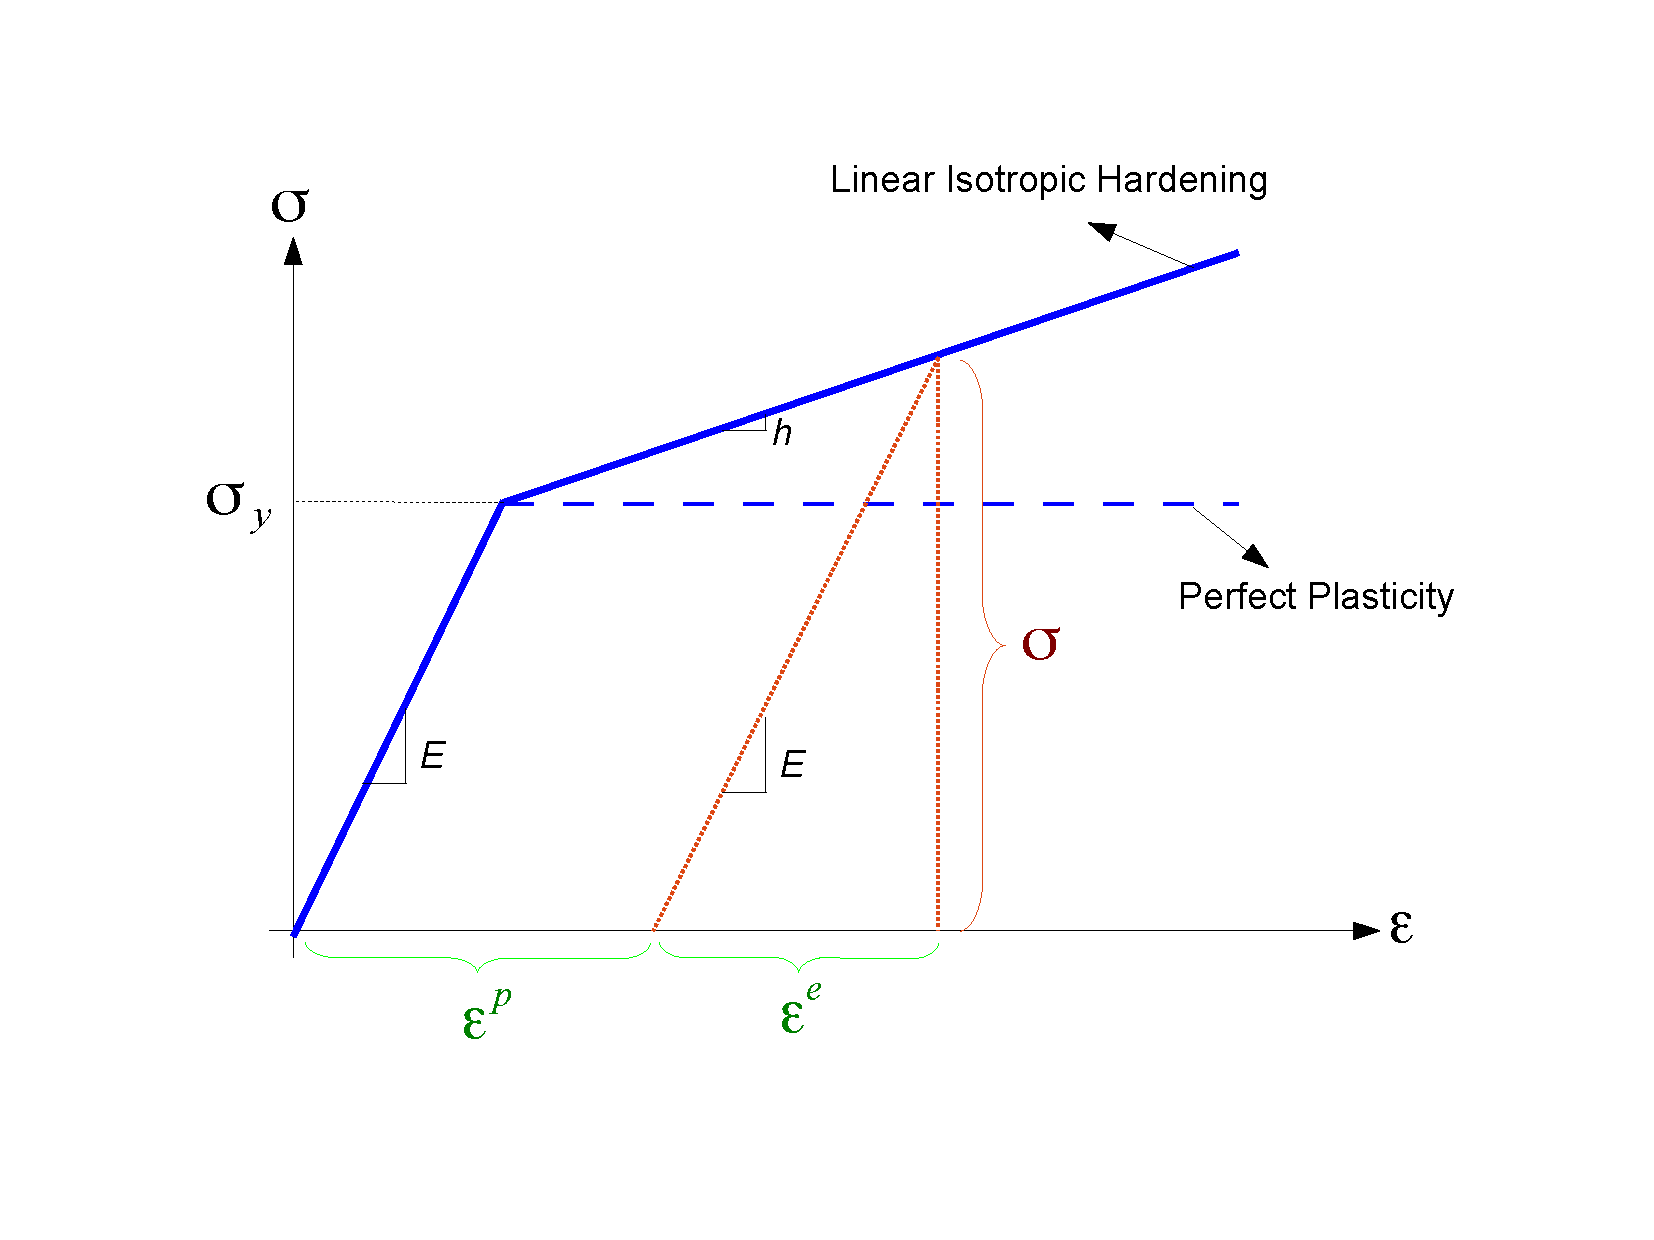
\includegraphics[scale=0.4, clip]{figures/isotropic_hardening_plasticity.pdf}}
   \caption{
    Stress-strain curve for the small-deformation plasticity with linear isotropic hardening.
   }
  \label{fig:smm:cl:Lin-strain-hard}
\end{figure}

\noindent In this class, the von Mises yield criterion is used. In the von Mises yield criterion, the yield is independent of the hydrostatic stress. Other yielding criteria such as Tresca and Gurson can be easily implemented in this class as well.

In the von Mises yield criterion, the hydrostatic stresses have no effect on the plasticity and consequently the yielding occurs when a critical elastic shear energy is achieved.

\begin{equation} \label{eqn:smm:constitutive:von Mises}
	f = \sigma_{\st{eff}} - \sigma_y = (\frac{3}{2} {\mat{\sigma}}^{\st{tr}} : {\mat{\sigma}}^{\st{tr}})^{1/2}-\sigma_y (\mat{\varepsilon}^p)
\end{equation}

\begin{equation} \label{eqn:smm:constitutive:yielding}
 	f < 0 \quad \textrm{Elastic deformation,} \qquad f = 0 \quad  \textrm{Plastic deformation}
\end{equation}

where $\sigma_y$ is the yield strength of the material which can be function of plastic strain in case of hardening type of materials and ${\mat{\sigma}}^{\st{tr}}$ is the deviatoric part of stress given by

\begin{equation} \label{eqn:smm:constitutive:deviatoric stress}
	{\mat{\sigma}}^{\st{tr}}=\mat{\sigma} - \frac{1}{3} trace(\mat{\sigma}) \mat {I}
\end{equation} 

After yielding $(f = 0)$, the normality hypothesis of plasticity determines the direction of plastic flow which is normal to the tangent to the yielding surface at the load point. Then, the tensorial form of the plastic constitutive equation using the von Mises yielding criterion (see equation 4.34) may be written as

\begin{equation} \label{eqn:smm:constitutive:plastic contitutive equation}
	\Delta {\mat{\varepsilon}}^p = \Delta p \frac {\partial{f}}{\partial{\mat \sigma}}=\frac{3}{2} \Delta p \frac{{\mat{\sigma}}^{\st{tr}}}{\sigma_{\st{eff}}}
\end{equation}

In these expressions, the direction of the plastic strain increment (or equivalently, plastic strain rate) is given by $\frac{{\mat{\sigma}}^{\st{tr}}}{\sigma_{\st{eff}}}$ while the magnitude is defined by the plastic multiplier $\Delta p$. This can be obtained using the \emph{consistency condition} which impose the requirement for the load point to remain on the yielding surface in the plastic regime.

\begin{table}[h]
\centering
  \begin{tabular}{| c | l | c |}
    \hline
    1 & Compute the trial stress & ${\mat{\sigma}}^{\st{tr}} = {\mat{\sigma}}_t + 2G\Delta \mat{\varepsilon} + \lambda trace(\Delta \mat{\varepsilon})\mat{I}$ \\[2ex] \hline
    2 & Check the Yielding criteria & $f = (\frac{3}{2} {\mat{\sigma}}^{\st{tr}} : {\mat{\sigma}}^{\st{tr}})^{1/2}-\sigma_y (\mat{\varepsilon}^p)$ \\[2ex] \hline
    3 & Compute the Plastic multiplier & \begin{tabular}{@{}c@{}c@{}} $d \Delta p = \frac{\sigma^{tr}_{eff} - 3G \Delta P^{(k)}- \sigma_y^{(k)}}{3G + h}		
$ \\ $\Delta p^{(k+1)}=\Delta p^{(k)}+ d\Delta p$ \\$\sigma_y^{(k+1)}=(\sigma_y)_t+ h\Delta p$ \end{tabular}\\ [2ex] \hline
    4 & Compute the plastic strain increment & $\Delta {\mat{\varepsilon}}^p = \frac{3}{2} \Delta p \frac{{\mat{\sigma}}^{\st{tr}}}{\sigma_{\st{eff}}}$ \\[2ex] \hline
    5 & Compute the stress increment & ${\Delta \mat{\sigma}} = 2G(\Delta \mat{\varepsilon}-\Delta \mat{\varepsilon}^p) + \lambda  trace(\Delta \mat{\varepsilon}-\Delta \mat{\varepsilon}^p)\mat{I}$ \\[2ex] \hline
    6 & Update the variables & \begin{tabular}{@{}c@{}} ${\mat{\varepsilon^p}}={\mat{\varepsilon}}^p_t+{\Delta {\mat{\varepsilon}}^p}$ \\    ${\mat{\sigma}}={\mat{\sigma}}_t+{\Delta \mat{\sigma}}$ \end{tabular}\\ [2ex] \hline     
    
  \end{tabular}
  \caption{Summary of the implementation procedure of small-deformation plasticity with linear isotropic hardening in \akantu}
  \label{table:equation for small-def plasticity with lin-iso-hardening}
\end{table}


Here, we summarize the implementation procedures for the
small-deformation plasticity with linear isotropic hardening. We use
an implicit integration technique called \emph{the radial return
  method} to obtain the plastic multiplier. This method has the
advantage of being unconditionally stable, however, the accuracy
remains dependent on the step size. The plastic parameters to indicate
in the material file are: \code{$\sigma_y$} (Yield stress) and
\code{h} (Hardening modulus). In addition, the elastic parameters need
to be defined as previously mentioned: \code{E} (Young's modulus),
\code{nu} (Poisson's ratio).


\subsection{Visco-Elasticity}

% Standard Solid rheological model, see [] J.C. Simo, T.J.R. Hughes,
% "Computational Inelasticity", Springer (1998), see Sections 10.2 and 10.3
Visco-elasticity is characterized by strain rate dependent
behavior. Moreover, when such a material undergoes a deformation it
dissipates energy. This dissipation results in a hysteresis loop in
the stress-strain curve at every loading cycle (see
Figure~\ref{fig:smm:cl:visco-elastic:hyst}). In principle, it can be
applied to many materials, since all materials exhibit a visco-elastic
behavior if subjected to particular conditions (such as high
temperatures).
\begin{figure}[!htb]
  \begin{center}

    \subfloat[]{
      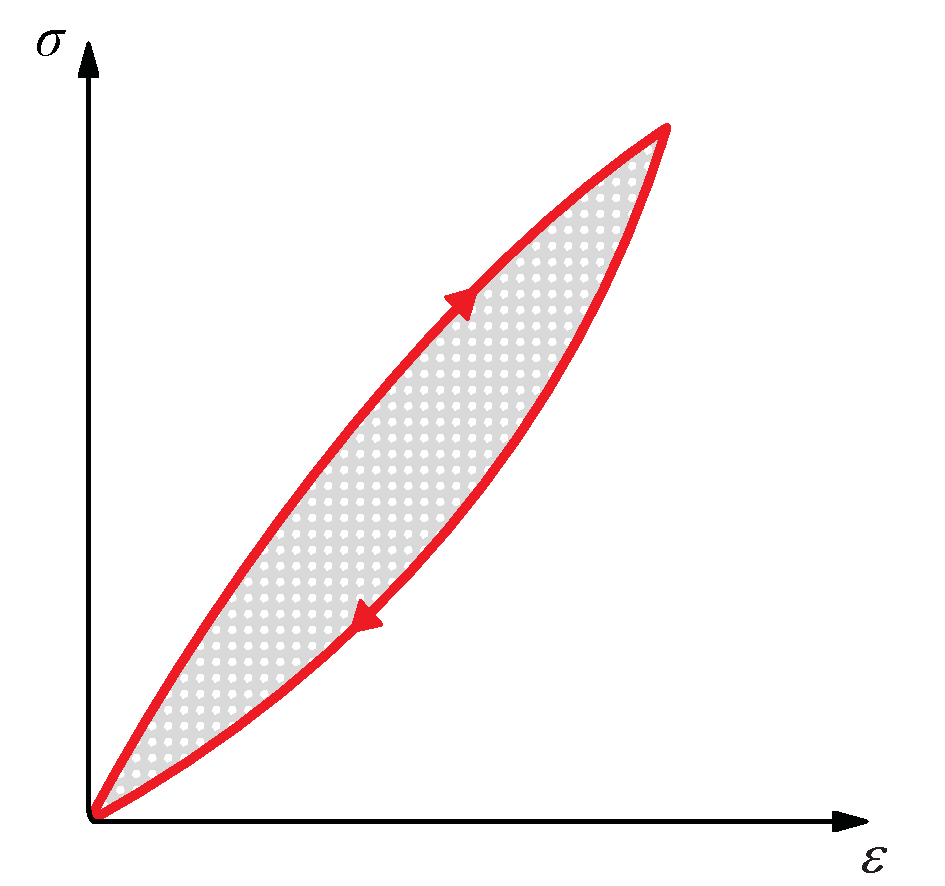
\includegraphics[width=0.4\textwidth,keepaspectratio=true]{figures/stress_strain_visco.pdf}
      \label{fig:smm:cl:visco-elastic:hyst}
    }
    \hspace{0.05\textwidth}
    \subfloat[]{
      \raisebox{0.025\textwidth}{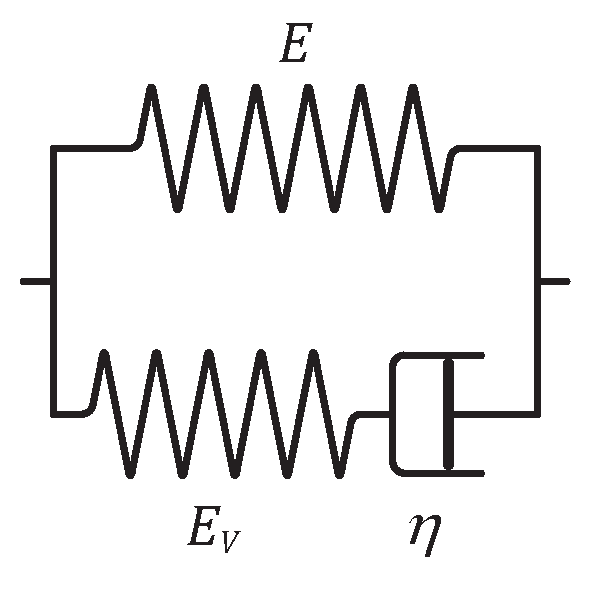
\includegraphics[width=0.3\textwidth,keepaspectratio=true]{figures/visco_elastic_law.pdf}}
      \label{fig:smm:cl:visco-elastic:model}
    }
    \caption{(a) Characteristic stress-strain behavior of a visco-elastic material with hysteresis loop and (b) schematic representation of the standard rheological linear solid visco-elastic model.}
    \label{fig:smm:cl:visco-elastic}
  \end{center}
\end{figure}
The standard rheological linear solid model (see Sections 10.2 and 10.3
of~\cite{simo92}) has been implemented in \akantu. This model results from the
combination of a spring mounted in parallel with a spring and a dashpot
connected in series, as illustrated in
Figure~\ref{fig:smm:cl:visco-elastic:model}. The advantage of this model is that
it allows to account for creep or stress relaxation. The equation that relates
the stress to the strain is (in 1D):
\begin{equation}
  \frac{d\epsilon(t)}{dt} = \left ( E + E_V \right ) ^ {-1} \cdot \left [ \frac{d\sigma(t)}{dt} + \frac{E_V}{\eta}\sigma(t) - \frac{EE_V}{\eta}\epsilon(t) \right ]
\end{equation}
where $\eta$ is the viscosity. The equilibrium condition is unique and
is attained in the limit, as $t \to \infty $. At this stage, the
response is elastic and depends on the Young's modulus $E$.  The
mandatory parameters for the material file are the following:
\code{rho} (density), \code{E} (Young's modulus), \code{nu} (Poisson's
ratio), \code{Plane\_Stress} (if set to zero plane strain, otherwise
plane stress), \code{eta} (dashpot viscosity) and \code{Ev} (stiffness
of the viscous element).

Note that the current standard linear solid model is applied only on the deviatoric part of the strain tensor. The spheric part of the strain tensor affects the stress tensor like an linear elastic material.

\subsection{Damage}

In the  simplified case of a  linear elastic and brittle  material, isotropic
damage can be represented by a scalar variable $d$, which varies from $0$ to $1$
for  no  damage  to  fully  broken  material  respectively.  The  stress-strain
relationship then becomes:
\begin{equation*}
  \mat{\sigma} = (1-d)\, \mat{C}:\mat{\varepsilon}
\end{equation*}

where  $\mat{\sigma}$,  $\mat{\varepsilon}$ are  the  Cauchy  stress and  strain
tensors, and $\mat{C}$ is the elastic stiffness tensor. This formulation relies
on the definition of an evolution law for the damage variable. In \akantu, many
possibilities exist and they are listed below.

\subsubsection{Marigo}
This damage evolution law is energy based as defined by Marigo \cite{marigo81a,
  lemaitre96a}. It is an isotropic damage law.
\begin{align}
  Y &= \frac{1}{2}\mat{\varepsilon}:\mat{C}:\mat{\varepsilon}\\
  F &= Y - Y_d - S d\\
  d &= \left\{
    \begin{array}{l l}
      \mathrm{min}\left(\frac{Y-Y_d}{S},\;1\right) & \mathrm{if}\; F > 0\\
      \mathrm{unchanged} & \mathrm{otherwise}
    \end{array}
  \right.
\end{align}
In this formulation, $Y$ is the strain energy release rate, $Y_d$ the
rupture criterion and $S$ the damage energy.  The non-local version of
this damage evolution law is constructed by averaging the energy $Y$.

\subsubsection{Mazars}
This law introduced by Mazars \cite{mazars84a} is a behavioral model to
represent damage evolution in concrete. The governing variable in this damage
law is the equivalent strain $\varepsilon_{\st{eq}} =
\sqrt{<\mat{\varepsilon}>_+:<\mat{\varepsilon}>_+}$, with $<.>_+$ the positive
part of the tensor.
The damage the is defined as:
\begin{align}
  D &= \alpha_t^\beta D_t + (1-\alpha_t)^\beta D_c\\
  D_t &= 1 - \frac{\kappa_0 (1- A_t)}{\varepsilon_{\st{eq}}} - A_t \exp^{-B_t(\varepsilon_{\st{eq}}-\kappa_0)}\\
  D_c &= 1 - \frac{\kappa_0 (1- A_c)}{\varepsilon_{\st{eq}}} - A_c
  \exp^{-B_c(\varepsilon_{\st{eq}}-\kappa_0)}\\
  \alpha_t &= \frac{\sum_{i=1}^3<\varepsilon_i>_+\varepsilon_{\st{nd}\;i}}{\varepsilon_{\st{eq}}^2}
\end{align}
With $\kappa_0$ the damage threshold, $A_t$ and $B_t$ the damage parameter in
traction, $A_c$ and $B_c$ the damage parameter in compression, $\beta$ is the
shear parameter. $\alpha_t$ is the coupling parameter between traction and
compression, the $\varepsilon_i$ are the eigenstrain and the
$\varepsilon_{\st{nd}\;i}$ are the eigenvalues of the strain if the material
were undamaged.

The coefficients $A$ and $B$ are the post-peak asymptotic
value and the decay shape parameters.


\subsection{Summary}\index{Material!List}

The list of all the materials available in Akantu is summarized in Tables \ref{tab:smm:cl:summary:list} as well as the keyword required for each material and the assosiated material properties.

\begin{table}[h!]
  \begin{center}
\begin{tabular}[c]{ m{3.5cm} | l | c | p{3.5cm} }
Material & Keyword & Parameter & Description \\
\hline
%%%%%%%%%%%%%%%%%
Linear elastic isotropic & \code{elastic} & -  & Table \ref{tab:smm:cl:summary:base}\\
\hline
%%%%%%%%%%%%%%%%%%
Linear elastic orthotropic  & \code{elastic\_orthotropic} & \code{Cij} & Tangent matrix coefficients (i,j = 1,2, ... voigt size ) \\
\hline
%%%%%%%%%%%%%%%%%%
Linear elastic anisotropic  & \code{elastic\_anisotropic} & \code{n1} & Direction of main material axis \\
 & & \code{n2} & Direction of secondary material axis \\
 & & \code{n3} & Direction of tertiery material axis \\
 & & \code{Cij} & Tangent matrix coefficients (i,j = 1,2, ... voigt size ) \\
 & & \code{alpha} & Proportion of viscous stress\\
\hline
%%%%%%%%%%%%%%%%%%
Neohookean (Finite-strain) \cite{Belytschko:2000} & \code{neohookean} & -  & Table \ref{tab:smm:cl:summary:base}\\
\hline
%%%%%%%%%%%%%%%%%%
Standard linear solid \cite{simo92} & \multirow{2}{*}{\code{sls\_deviatoric}} & - & Table \ref{tab:smm:cl:summary:base}\\
 & &  \code{Eta} & Viscosity\\
 & & \code{Ev} & Stiffness of the viscous element \\
\hline
%%%%%%%%%%%%%%%%%%
Elasto-plastic linear isotropic hardening & \code{plastic\_linear\_isotropic\_hardening}  & - & Table \ref{tab:smm:cl:summary:base}\\
 & &  \code{h} & Hardening modulus\\
 & &  \code{sigma\_y} & Yielding stress\\
\hline
%%%%%%%%%%%%%%%%%%
Visco-plastic & \code{visco\_plastic}  & - & Table \ref{tab:smm:cl:summary:base}\\
 & &  \code{rate} & Rate sensitivity component\\
 & &  \code{edot0} & Reference strain rate\\
 & &  \code{ts} & Time \\
\hline
\end{tabular}
\end{center}
  \caption{List of material properties with their corresponding keywords and material parameters.}
  \label{tab:smm:cl:summary:list}
\end{table}

\vspace{0.5cm}

In addition to the properties presented in Table \ref{tab:smm:cl:summary:list}, every material also has the parameter ''\code{rho}`` which corresponds to the density. The properties listed in Table  \ref{tab:smm:cl:summary:base} correspond to the parameters required to describe a linear elastic isotropic material, however those parameters are also commun to most of the materials available as previously described in Table \ref{tab:smm:cl:summary:list}.

\begin{table}[h!]
  \begin{center}
\begin{tabular}[c]{  l | p{6.5cm} }\label{tab:smm:cl:summary:base}
Parameter & Description \\
\hline
%%%%%%%%%%%%%%%%%
\code{rho}  & Density\\
\code{E}  & Young's modulus\\
\code{nu}  & Poisson's ratio\\
\code{Plane\_Stress} & Plane stress simplification (only 2D problems)\\
\hline
\end{tabular}
\end{center}
  \caption{List of material parameters shared my most materials}
  \label{tab:smm:cl:summary:base}
\end{table}

%%% Local Variables:
%%% mode: latex
%%% TeX-master: "manual"
%%% End:
}{}

\IfFileExists{manual-cohesive_element.tex}{
\subsection{Cohesive laws\todo{Marco}}

\subsubsection{Exponential cohesive law}

Ortiz and Pandolfi proposed this cohesive law in 1999 \ref{ortiz1999}.  The
traction-opening equation for this law is as following:

\begin{equation}
  \label{eq:exponential_law}
  t = e \sigma_c \frac{\delta}{\delta_c}e^{-\delta/ \delta_c}
\end{equation}


This equation is plotted in figure (\ref{fig:smm:CL:ECL}).

 \begin{figure}[!htb]
    \begin{center}
      \includegraphics[width=0.6\textwidth,keepaspectratio=true]{figures/cohesive_exponential.pdf}
      \caption{Exponential cohesive law}
      \label{fig:smm:CL:ECL}
    \end{center}
  \end{figure}



\subsubsection{Static cohesive element}

For  the  static  analysis   of  the  structures  containing  cohesive
elements, the stiffness of the cohesive elements should also be added to the
total      stiffness       of      the      structure.      Therefore,
the  function  \code{assembleStiffnessMatrix}  is written  in  the
\code{MaterialCohesive}.

Considering a typical cohesive element as explained in figure ???, the opening
displacement along the mid-surface can be written as:

\begin{equation}
  \label{eq:opening}
  \delta(\xi) = [[\mat{u}]] \mat{N}(\xi) =
\begin{bmatrix}
u_3-u_0 & u_4-u_1 & u_5-u_2\\
v_3-v_0 & v_4-v_1 & v_5-v_2
\end{bmatrix}
\begin{bmatrix}
N_0(\xi) \\ N_1(\xi) \\ N_2(\xi)
\end{bmatrix} =
\mat{N A U}
\end{equation}

 The \mat{U} , \mat{A} and \mat{N} are as following:

\begin{equation}
  \mat{U} = \left [
\begin{array}{c c c c c c c c c c c c}
u_0 & v_0 & u_1 & v_1 & u_2 & v_2 & u_3 & v_3 & u_4 & v_4 & u_5 & v_5
\end{array}\right ]
\end{equation}


\begin{equation}
  \mat{A} = \left [\begin{array}{c c c c c c c c c c c c}
1 & 0 & 0 & 0& 0 & 0 & -1& 0 & 0 &0 &0 &0\\
0 &1& 0&0 &0 &0 &0 & -1& 0& 0 & 0 &0\\
0 &0& 1&0 &0 &0 &0 & 0& -1& 0 & 0 &0\\
0 &0& 0&1 &0 &0 &0 & 0& 0& -1 & 0 &0\\
0 &0& 0&0 &1 &0 &0 & 0& 0& 0 & -1 &0\\
0 &0& 0&0 &0 &1 &0 & 0& 0& 0 & 0 &-1
\end{array} \right ]
\end{equation}


 \begin{equation}
 \mat{N} = \begin{bmatrix}
N_0(\xi) & 0 & N_1(\xi) &0 & N_2(\xi) & 0\\
0 & N_0(\xi)& 0 &N_1(\xi)& 0 & N_2(\xi)
\end{bmatrix}
\end{equation}

The consistent stiffness matrix for the element is obtained as

\begin{equation}
  \label{eq:cohesive_stiffness}
  \mat{K}    =    \delta    \mat{U}^T    \int_{\Gamma_c}    {\mat{P}^t
    \frac{\partial{\mat{t}}} {\partial{\delta}} \mat{P} d
    \Gamma \Delta \mat{U}}
\end{equation}

In which the  tangent matrix is calculated based  on the equation \ref
{eq:tangent_cohesive} after
performing necessary derivation:

\begin{equation}
  \label{eq:tangent_cohesive}
   \frac{\partial{\mat{t}}} {\partial{\delta}} = \hat{\mat{t}} \otimes
   \frac                       {\partial{(t/\delta)}}{\partial{\delta}}
   \frac{\hat{\mat{t}}}{\delta}+ \frac{t}{\delta}  [ \beta^2 \mat{I} +
   (1-\beta^2) (\mat{n} \otimes \mat{n})]
\end{equation}

 In which $\frac{\partial{(t/\delta)}}{\partial{\delta}}$ in the first
 term is

\begin{equation}
 \frac{\partial{(t/ \delta)}}{\partial{\delta}} = \left\{\begin{array} {l l}
-e  \frac{\sigma_c}{\delta_c^2  }e^{-\delta  /  \delta_c} &  \quad  if
\delta \geq \delta_{max}\\
 0 & \quad if \delta < \delta_{max}, \delta_n > 0
\end{array} \right.
\end{equation}

This      tangent      matrix      is     implemented      in      the
\code{computeTangentStiffness} function for
the exponential law.

A full example for the static analysis of the cohesive elements can be
found in \code{\examplesdir/static\_cohesive}.

%%% Local Variables:
%%% mode: latex
%%% TeX-master: "manual"
%%% End:
}{}

\section{Adding a new constitutive law}\index{Material!create a new
material}

There are several constitutive laws in \akantu as described in the
previous Section \ref{sect:smm:CL}. It is also possible to use a
user-defined material for the virtual simulation. These materials will
be referred to as local materials since they are local to the example
of the user and not part of the akantu library.  To define a new local
material, two files (\code {material\_XXX.hh} and
\code{material\_XXX.cc}) should be provided where \code{XXX} is the
name of the new material. Define the interface of your custom material
in \code{material\_XXX.hh} and its implementation in
\code{material\_XXX.cc}.  The new law must inherit from the
\code{Material} class or any other existing material class and the
following functions have to be redefined for the new constitutive law:

\begin{cpp} void initMaterial();

  // for explicit and implicit simulations void
computeStress(ElementType el_type, GhostType ghost_type = _not_ghost);

  // for implicit simulations void computeTangentStiffness(const
ElementType & el_type, Array<Real> & tangent_matrix, GhostType
ghost_type = _not_ghost);

  // for explicit and implicit simulations Real getStableTimeStep(Real
h, const Element & element);
\end{cpp} These functions will be explained in detail at the end of
this section.  For each material, the minimum required parameters have
to be defined in a material file.  For existing materials, as
mentioned in section \ref{sect:smm:CL}, the materials are initialized
by default inside the function \code{initFull}. If a local material
should be used the initialization of the materials has to be postponed
until the local material is registered in the model. Therefore, the
model is initialized with the boolean for skipping the material
initialization equal to true:
\begin{cpp} /// model initialization
  model.initFull(SolidMechanicsModelOptions(_explicit_lumped_mass,
  true));
\end{cpp} Once the model has been initialized the local material needs
to be registered in the model. In order to register all the material
parameters correctly, these parameters need to be defined in the
constructor of the class with the function
\code{registerParam}\index{Material!registerParam}:
\begin{cpp} 
  void registerParam(name of the parameter (key in the
  material file), member variable, default value (optinal parameter),
  access permissions description);
\end{cpp} Moreover, some internal values can be considered for each
quadrature point. An example for such an internal value could be the
damage on each quadrature point. Since the number of quadrature points
depends on the element type, these internal values are stored in a
\code{ElementTypeMapReal}. The internal values, like all class
members, are declared in the \code{material\_XXX.hh} file:
\begin{cpp} 
  /// damage internal variable 
  InternalField<Real> damage;
\end{cpp} 
and they are initialized in the constructor of the new law with
the function \code{initialize}\index{Material!initialize}:
\begin{cpp} 
  damage.initialize(1);
\end{cpp} Here, the value $1$ corresponds to the number of components,
in this case one value per quadrature point. The internal values can
be resized to the current number of quadrature points at any time with
the function \code{resize}\index{Material!resize}.  Then the material
can be registered in the model by calling the function
\code{registerNewCustomMaterial}:
\begin{cpp}
model.registerNewCustomMaterials<XXX>("name_of_local_material");
\end{cpp} In the following, the functions that have to be redefined
will be described in detail:
\begin{itemize}

\item \code{initMaterial}:~ This function is called after the material
file is fully read and the elements corresponding to each material are
assigned. Some of the frequently used constant parameters are
calculated in this function. For example, the Lame's constants of
elastic materials can be considered as such parameters.

\item \code{computeStress}:~ In this function, the stresses are
computed based on the constitutive law knowing the strains for the
quadrature points.  For example, the stresses for the elastic material
are calculated based on the following formula:
  \begin{equation}\label{eqn:smm:constitutive_elastic} \mat{\sigma }
=\lambda\mathrm{tr}(\mat{\varepsilon})\mat{I}+2 \mu \mat{\varepsilon}
  \end{equation}

  Therefore, this function contains a loop on all quadrature points
assigned to the material using the
\code{MATERIAL\_STRESS\_QUADRATURE\_POINT\_LOOP\_BEGIN;} and
\code{MATERIAL\_STRESS\_QUADRATURE\_POINT\_LOOP\_END;} macros.

  \begin{cpp} MATERIAL_STRESS_QUADRATURE_POINT_LOOP_BEGIN;

    // sigma <- f(grad_u)

    MATERIAL_STRESS_QUADRATURE_POINT_LOOP_END;
  \end{cpp}

  \note{The strain vector in \akantu contains the values of $\nabla
\vec{u}$.}

\item \code{computeTangentStiffness}:~ This function is called when
the tangent to the stress-strain curve is desired (see Fig \ref
{fig:smm:AL:K}).  For example, it is called in the implicit solver
when the stiffness matrix for the regular elements is assembled based
on the following formula:
  \begin{equation} \label{eqn:smm:constitutive_elasc} \mat{K }
=\int{\mat{B^T}\mat{D(\varepsilon)}\mat{B}}
  \end{equation}

  Therefore, in this function the \code{tangent} matrix (\mat{D}) is
computed for a given strain.

  \note{ The \code{tangent} matrix is a $4^{th}$ order tensor which is
stored as a matrix in the Voigt notation.}

  \begin{figure}[!htb]
    \begin{center}
      \includegraphics[width=0.4\textwidth,keepaspectratio=true]{figures/tangent.pdf}
      \caption{Tangent to the stress-strain curve.}
      \label{fig:smm:AL:K}
    \end{center}
  \end{figure}


\item \code{getStableTimeStep}:~ The stable time step should be
calculated based on \eqref{eqn:smm:explicit:stabletime} for the
explicit methods.  This function depends on the longitudinal wave
speed which changes for different materials and strains. Therefore,
the value of this velocity should be defined in this function for each
new material.

  \note {In case of need, the calculation of the longitudinal and
shear wave speeds can be done in separate functions
(\code{getPushWaveSpeed} and \code{getShearWaveSpeed}).  Therefore,
the first function can be called for calculation of the stable time
step.}
\end{itemize}

A full example for adding a new damage law can be found in
\shellcode{\examplesdir/new\_material}.

%%% Local Variables: %%% mode: latex %%% TeX-master: "manual" %%% End:
